\documentclass[twoside,openright,a4paper,11pt,french]{article}
\usepackage[utf8]{inputenc}
\usepackage[french]{babel}
\usepackage[T1]{fontenc}
\usepackage{emptypage}
\usepackage{amsmath}

% Utilisation d'url
\usepackage{url}
\urlstyle{sf}

% Utilisation d'images, stockées dans le répertoire ./pics/
\usepackage{graphicx}
\graphicspath{pics/}

% Définition des marges
\usepackage{geometry}
\geometry{
  left=25mm,
  right=25mm,
  top=25mm,
  bottom=25mm,
  foot=15mm
}
\usepackage{listings}
\usepackage{color}

\definecolor{gray}{rgb}{0.8,0.8,0.8}

\begin{document}

\pagestyle{plain}
\setlength{\parindent}{0pt}
% La page de garde
\thispagestyle{empty}

\begin{center}
       \noindent
       
\includegraphics[height=2.5cm]{./pics/uds.eps}       
       
       \vfill\vfill

    {\large \textsc{Licence 3 de Sciences, mention Informatique}}

    \bigskip\bigskip

    {\large \textsc{Programmation Orientée Objet 2 }}

    \vfill\vfill

% Titre du document
    {\huge \sc
      \begin{center} 
        Rapport sur le projet: \\
        détection des bords et vectorisation
      \end{center}}

    \vfill\vfill

    {\large Présenté par}

\medskip

% Identité des auteurs
    {\large Victor \textsc{Constans}}\\
    {\large Luigi  \textsc{Coniglio}}\\
\bigskip

\end{center}



% La table des matières
\parskip=0pt
\tableofcontents


\vspace{5cm}

%Start content

\section{Fichiers rendus et usage}
\subsection{Contenu du rapport}
L'objectif de ce rapport est d'abord d'illustrer la structure du
programme. Pour accelérer/simplifier l'utilisation du travail rendu, la partie
initiale de ce rapport décrit le contenu des fichiers et leur usage.

\subsection{Contenu de l'archive}
Après avoir ouvert l'archive {\it constans\_coniglio\_luigi.tar.gz} vous
trouverez les fichiers et répertoires suivants:
\smallbreak
\begin{itemize}
\item Ce rapport
\item Le fichier {\bf javimy.java} qui est le point d'entrée du programme
\item Les répertoires {\bf window} et {\bf option} qui contiennent tous les fichiers du programme relatifs
      à l'interface graphique
\item Le répertoire {\bf filters} qui contient un package incluant tous les filtres 
      implementés dans la cadre de ce projet
\item Le répertoire {\bf vectorization} qui contient la partie du programme dédiée à
      la vectorisation d'une image
\end{itemize}

\section{Répartition des tâches}
La majorité des algorithmes implémentés dans ce projet ont été pensés par l'ensemble du groupe.
Cependant, la production du code à été répartit comme suit:
\begin{itemize}
\item {\bf Luigi CONIGLIO}: Filtre de Sobel, segmentation, filtre Cluster-Edges, vectorisation
\item {\bf Victor CONSTANS}: Interface graphique, filtre de Prewitt, Gauss, Roberts, Kirsch, Canny
\end{itemize}


\bigbreak
\subsection{Usage}
Compiler le programme par le biais de la commande : 
\colorbox{gray}{\lstinline[basicstyle=\ttfamily\color{black}]| make |}
Une fois la création des fichiers{\it .class} terminé vous êtes prêt
à utiliser ce magnifigue logiciel: 
\colorbox{gray}{\lstinline[basicstyle=\ttfamily\color{black}]| java javimy |},

\vspace{1cm}
A l'exécution, il vous sera présenté une interface graphique qui vous
permettra de façon assez intuitive d'accéder aux differentes fonctions
du programme:

\begin{center}
% TODO image GUI %
\end{center}

\newpage 
\section{Implémentation}
Voyons maintenant l'implémentation et la structure du programme.
Cette structure peut être divisée en trois sections que sont:
\begin{itemize}
\item l'interface graphique
\item les filtres
\item la vectorisation
\end{itemize}

\begin{figure}[h]
\centering
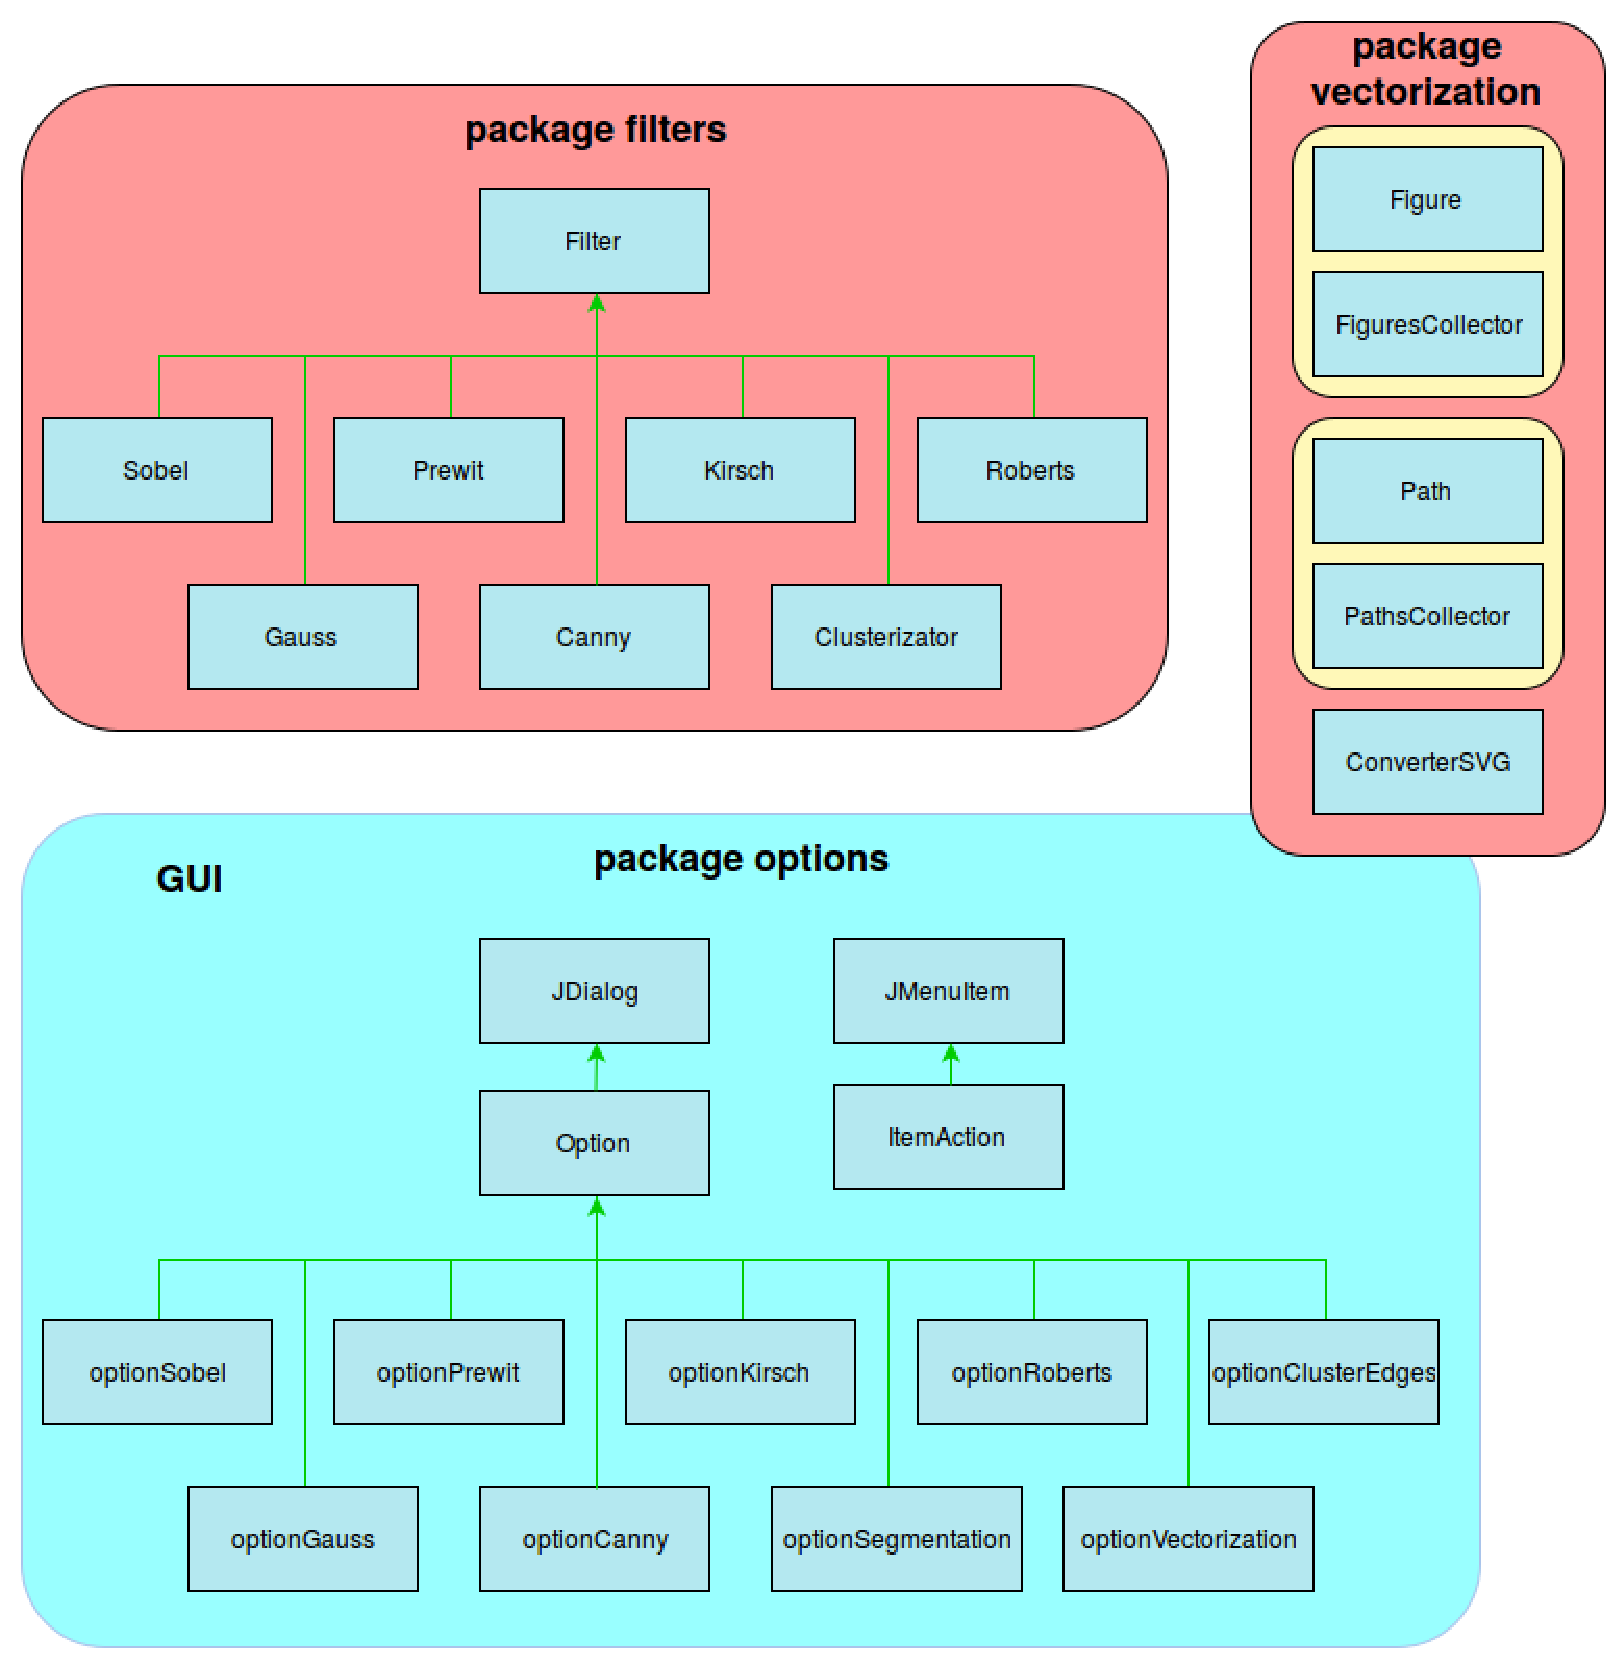
\includegraphics[width=12cm]{./pics/classes.eps}
\caption{Diagramme d’heritages et de classes}
\end{figure}


Comme nous pouvons le voir sur le diagramme ci-dessus, l'interface graphique à une hiérarchie
particulière. En effet, cela à été fait pour permettre d'appeler le bon filtre de manière la
plus générique possible: à savoir, lancé l'execution de l'objet correspondant au filtre que l'on
souhaite appliqué sans avoir à distinguer de cas pour chaque filtre.
De cette manière si on souhaite ajouter un filtre, il suffit d'ajouter le bouton d'execution de
se filtre et de créer un fichier option (que nous allons détailler) sans avoir à ajouter de traitement
particulier pour ce filtre. Voyons plus précisement cette implémentation.
Lorsque l'on ajoute un filtre, on va lui attribuer un ItemAction qui est une classe étendue de MenuItem.
ItemAction permet de profiter des fonctionnalités de MenuItem, mais il permet de rajouter comme attribut,
un objet Option qui permettra de paraméttrer et d'executer le bon filtre. Donc lors de la création d'un
ItemAction, on passe un objet (Option) qui correspond aux paramétrage et au stockage du filtre qu'il faudra
executer lorsque l'on cliquera sur ce button.
La classe Option est une classe abstraite qui permet de regrouper sous un parent toute les différentes classes
spécifique au filtre. Elle dérive de la classe JDialog qui permet de profiter d'un affichage des options à
l'écran, affichage qui a la particularité d'avoir un affichage bloquant. L'avantage est que cela empêche la
fenêtre principale de continuer son execution et de tenter d'afficher une image filtrer alors qu'elle n'a pas
encore été calculée. Avec ce système, lorsqu'une fenêtre d'option de filtre s'ouvre, elle bloque l'execution
de la fenêtre principale, cela permet à la fenêtre option de filtre de receuillir les options demandé à
l'utilisateur et de filtrer l'image. Une fois l'execution du filtre terminée, la fenêtre est retiré de l'affichage
ce qui libère la fenêtre principale qui pourra alors récupérer l'image filtrer et l'afficher à l'écran.
Cette classe va aussi regrouper les attributs et méthode générique aux différents filtres, en particulier une
variable contenant l'image filtrer, l'image source, un panel qui va contenir les différents
éléments affiché à l'écran et un boutton submit qui permet de valider
les options que l'on a rentrer et de lançer l'execution du filtre.
Enfin, les différentes classes option de filtre (optionSobel, optionPrewitt, ...) sont les derniers maillons qui
vont contenir les différentes options qui vont être demandées à l'utilisateur (typiquement des seuils) ainsi que
l'appel à la fonction de filtre.
Lorsque l'utilisateur pas presser un bouton de filtre, action va être lu par la fenêtre principale, qui va recupérer l'objet 
à l'origine de l'action (ici un ItemAction) et elle va appeller la méthode affiche de cette objet, qui va lançer l'affichage
des options. Une fois que l'utilisateur valide ses options le filtre s'execute.

La deuxième section est celle des filtres. Elle est constitué d'une classe abstraite Filter qui permet de regrouper les
attributs communs aux différents filtres.
Les différentes classe de filtre étende cette classe Filter de sorte que les filtre apparaissent sous un objet unique; un Filter.

Les classes de la partie vectorisation n'ont pas de lien hiérarchique entre
eux. Cependant les objets de cette section sont complémentaires étant qu'il y a un lien de producteur/consommateur.


\section{Filtres}
\label{sec:filtres}

\subsection{Sobel, Prewitt, Roberts et Kirsch}
Les algorithmes utilisés dans ce projet (à savoir Sobel, Prewitt, Roberts et Kirsch)
fonctionnent tous sur le principe de convolution de pixel avec une matrice.
Le principe est que l'on va appliquer une (ou plusieurs) matrices de convolution propre
à chaque filtre, sur les pixels de l'image. Nous allons donc superposer la matrice sur
l'image avec en son centre le pixel que l'on traite, et on multiplie la valeur du pixel
par le coefficient se trouvant "au dessus du pixel" dans la matrice. On somme tous les
produits issus de la convolution avec la matrice et l'on obtient la nouvelle valeur du pixel.

Dans les filtres que nous utilisons, nous faisons deux convolutions, avec deux
matrices différentes qui vont analyser les alentours du pixel de manière
horizontale pour l'une et verticale pour l'autre. Nous obtenons donc deux
gradients (X et Y) dont nous pouvons estimer la norme une fois combiné avec la
formule:
$\sqrt[2]{X^2+Y^2}$

Nous appliquons un coefficient, issus de la valeur du plus grand pixel après la convolution,
pour avoir une valeur comprise entre 0 et 255, et cela nous donne la nouvelle valeur du pixel.

Sobel, Prewitt et Roberts fonctionnent de cette manière; seul les valeurs et
les dimensions des matrices de convolution change.
Kirsch fonctionne aussi de cette façon, seulement il va appliquer 8 matrices de convolution
représentant les 8 directions entourant le pixel, et il va retenir la valeur de convolution
la plus haute.

\subsection{Canny}
L'algorithme de Canny utilise aussi le principe de convolution mais de manière plus évolué.
En effet, l'image est d'abord traitée avec un filtre de \ref{Gauss} afin de réduire le bruit et
la rendre plus lisse.
Dans un second temps nous utilisons une convolution habituelle pour obtenir des gradient, mais cette fois-ci
nous obtenons aussi la direction du gradient. Nous arrondissons les angles que formes des gradient par rapport
à l'axe horizontale avec un pas de 45°.
Il faut à présent supprimer les points non-maxima local par rapport au masque de convolution, qui pourrait
élargir les bords si on les laissaient. On va donc pour cela, chercher les valeurs des pixels se trouvant "sous"
la matrice de convolution qui sont plus grande que la valeur du pixel qui l'on traite, et dont la direction est
la même que le pixel que l'on est entrain de traiter. Si on trouve un tel pixel, alors le pixel courant ne 
sera pas retenu et mis à un état invalide.
A partit de là nous n'avons plus que les maxima-locaux, donnant un bord bien net, il ne reste plus
qu'à sueiller les pixels qui sont encore valides. Pour qu'un pixel soit valide il faut que son intensité soit
élevé, ce qui signifie qu'il y a un bord à cet endroit. On utilise deux seuils qui vont définir si un pixel
peut être compter comme étant un bord. En dessus du seuil minimum, le pixel n'est mis dans un état invalide,
car son intensité n'est pas assez élevée pour être considéré comme un bord. Si elle est au dessus du seuil
maximum alors on estime que le pixel peut être considéré comme un bord. Entre ces deux seuils, on ne peux pas
vraiement savoir si un pixel est effectivement un bord ou non. On va donc simplement regarder les voisins directe
de ce pixel, et si un ceux-ci est valide et considéré comme un bord, alors le pixel courant est aussi considéré
comme un bord.

\subsection{Gauss}
\label{sec:gauss}
%TODO Description du principe de fonctionnement avec quelque image/example
L'algorithme utilisé pour le lissage d'image est l'algorithme de Gauss. Celui-ci va générer une
matrice de convolution à l'aide d'une formule mathématique. Il va ensuite, comme les autres filtre,
appliqué une convolution avec le matrices généré. La subtilité par rapport aux autres fitre, et qu'ici
il faut déterminer la valeur maximal des trois composantes RVB pour appliquer un coefficient
permettant rester dans la plage 0-255 sur les 3 composantes.

\subsection{Segmentation}
La segmentation a pour objectif de partitionner une image en sections
(ensembles de pixels) sur la base de leurs propriétés (couleurs,
intensité, ...). Dans le menu des filtres vous trouverez un bouton qui
vous permettra de réaliser ce type d'opération sur les couleurs
d'une image.

L'algoritme utilisé pour segmenter l'image est inspiré du
partitionnement en {\it K-moyennes} (ou {\it k-means clustering} en
anglais). Ce type de partitionnement consiste à sélectioner K couleurs
et à assigner à chaque pixel de l'image à la plus proche de ces couleurs.

\begin{figure}[h]
\centering
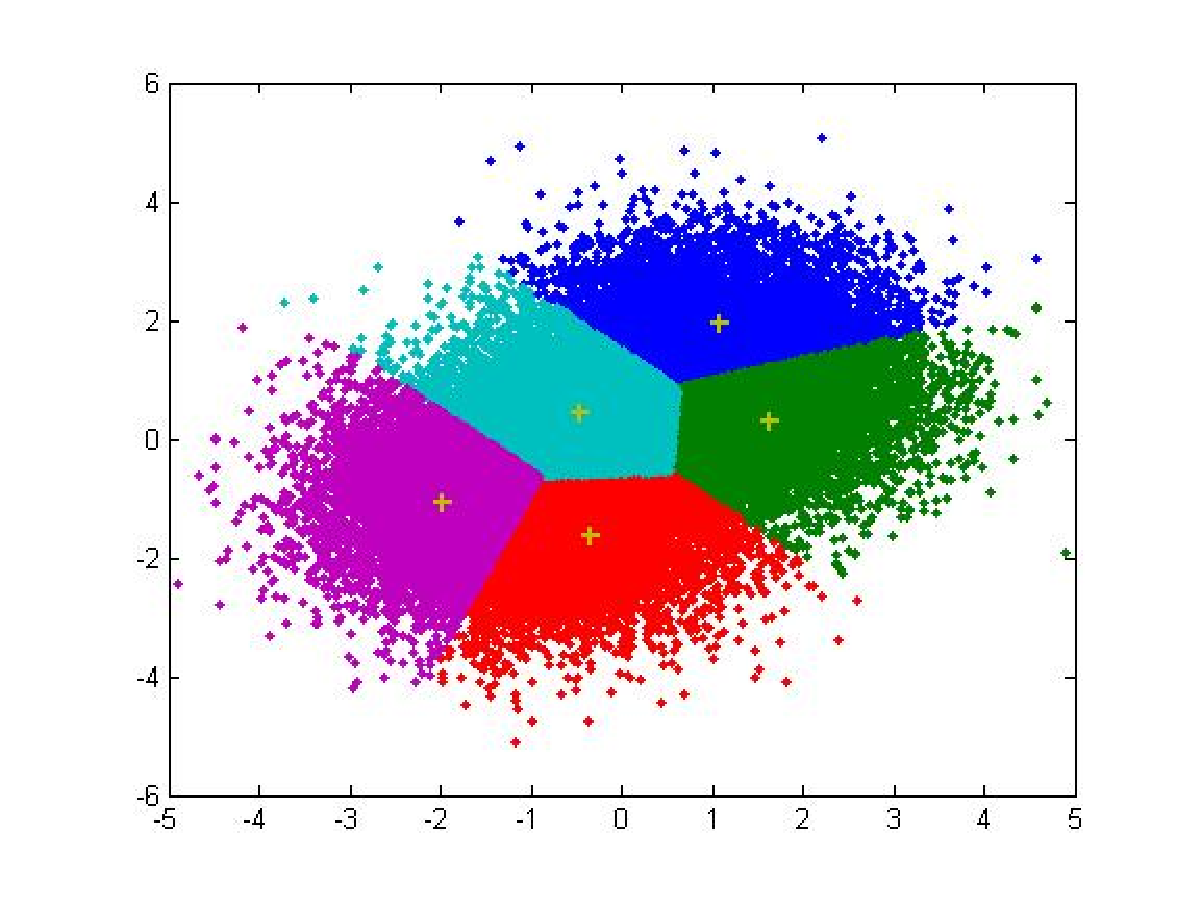
\includegraphics[width=8cm]{./pics/kmeans.eps}
\caption{Agrégation des pixels selon la plus courte distance avec les
K-moyennes (ici K = 5)}
\label{fig:routcidr}
\end{figure}

Les K couleurs vont ensuite êtres modifiées pour prendre comme valeur la
moyenne de la couleur des pixels qui lui sont associés, dans le but de
minimiser l'écart de couleur avec les pixels de l'image. Cette opération va
être répétée jusqu'à ce que les K couleurs et le partitionnement des pixels
convergent. 

\subsection{Cluster-edges}
Ce filtre s'inscrit dans l'ensemble des filtres de détections des
bords. La particularité de ce filtre vis-à-vis des autres filtres de
détection des contours est qu'il n'effectue pas qu'une simple détection
des bords mais. En effet, il détermine plus précisement les limites entre les
différentes zones de couleurs. 
La limite entre deux zones de couleurs est représentée par des
chemin coloré. A chaque bord correspond un chemin d'une couleur
différente \cite{url-novelvect}.

Le première étape de l'algoritme consiste à segmenter l'image en
différentes zones de couleurs.

\begin{figure}[h]
\centering
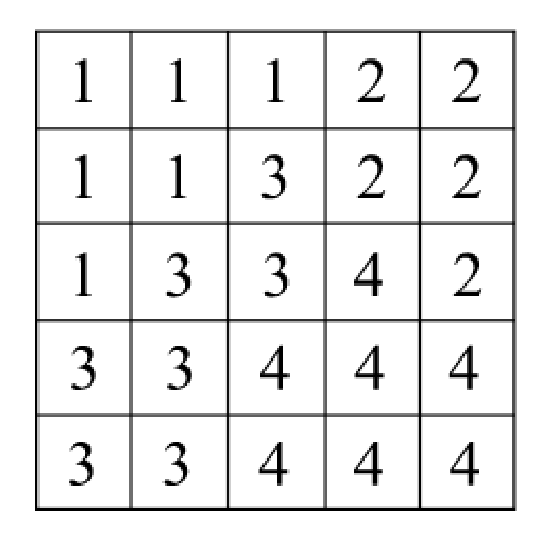
\includegraphics[width=3.5cm]{./pics/cluster-edges1.eps}
\caption{Segmentation, chaque nombre représente une couleur differente}
\label{fig:routcidr}
\end{figure}

Une fois la segmentation terminée on procède à la génération de
sub-pixels entre chaque pixel de l'image originale. Chaque sub-pixel
est rempli selon la couleur des pixels autour de lui.

\begin{figure}[h]
\centering
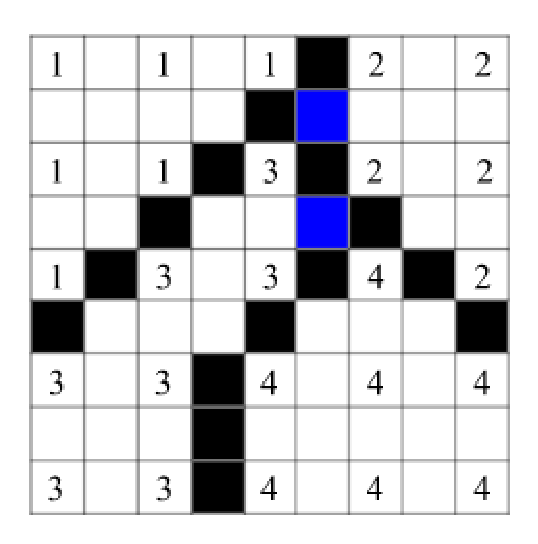
\includegraphics[width=3.5cm]{./pics/cluster-edges2.eps}
\caption{Les bords sont les sub-pixel ayant comme voisins des pixels de
couleur différente}
\label{fig:routcidr}
\end{figure}

\newpage

\section{Vectorisation} 
Le programme permet d'exporter une image sous la forme d'un fichier
{\it .svg}. La conversion d'une image dans le format SVG ({\it
Scalable Vector Graphics}) suit un processus assez complexe qui ne vaut
pas la peine d'être présenté.

Si la plupart des formats représentant une image en utilisant un 
mappage plus ou moins complexe de pixel, un format d'image vectorielle
permet de représenter une image comme etant un ensemble de formes
egendre par des vecteurs. Vectoriser une image consiste à traduire
l'ensemble des pixels d'une image en vecteurs (formes géométriques,
chemins, courbes, etc ...).

L'algorithme utilisé pour vectoriser une image dans le cadre de ce projet peut
être résumé par les étapes suivantes:   

\smallbreak
\begin{itemize}
\item Segmentation de l'image
\item Détection des contours et extraction des bords
\item Compression des bords
\item Construction des figures
\item Conversion au format SVG
\end{itemize}   
\bigbreak

La segmentation et la détection des contours d'une image sont effectuées
en utilisant les techiques présentes dans la section
\ref{sec:filtres} de ce rapport.


\subsection{Compression des contours}
%TODO Algorithme de Douglas-Peucker %
Au moment de la détection, chaque bord est extrait comme étant une
suite continue de pixels. Bien qu'une telle représentation soit tout à
fait utilisable dans la construction d'une image vectorielle le
resultat ne serait pas très différent de celui d'un format standard
d'image. C'est pour cette raison que pendant le processus de vectorisation d'une
image, les suites continues de pixels constituant les contours de
l'image doivent être traduits comme des éléments géométriques plus
simples: segments, courbes, etc.. .  

La première étape dans la traduction des contours consiste à réduire
le nombre de pixels. Dans la cadre de ce projet nous avons décidés d'utiliser
l'algorithme de Douglas-Peucker pour atteindre cet objectif
\cite{url-dougpeuck}.

L'algorithme de Douglas-Peucker est beaucoup utilisé en géographie pour
l'approximation des trajet et permet de réduire les points d'un chemin en
tenant compte d'un certain degré de liberté (paramétrable).

\begin{figure}[h]
\centering

\includegraphics[width=7cm]{./pics/dp1.eps}
\caption{Les bords sont approximés avec un degré de liberté croissant}
\label{fig:routcidr}
\end{figure}

Le fait que cet algorithme soit facilement paramétrable a été un élément clé
dans le choix de celui-ci, et il permet a l'utilisateur de choisir la précision
souhaité dans la vectorisation.

Un autre élément essentiel dans le choix de cet algorithme a été le
fait que il ne change pas la position du premier et du dernier point
d'un chemin dans la compression de celui-ci. Grâce à cela, un chemin
(partie d'un contour) d'une image commencera et terminera toujours sur
le en un même point, même après la compression, et assurant ainsi la
contiguité de celui-ci avec les bords voisins.



\subsection{Construction des figures}
%TODO voisinage de moore %
Une fois les contours simplifiés, arrive le moment de traiter
les zones de couleurs engendré par les bords.

On peut définire une {\it figure} comme étant une section de l'image ayant
(après segmentation) une unique couleur, et qui engendre la combinaison de
plusieurs bords.

Le but à ce stade est de détecter toutes les {\it figures} de l'image et
d'afféeter à chaque {\it figure} les bords entourant celle-ci dans le
bon ordre (sachant qu'un bord est toujours partagé entre deux
{\it figures}).

L'algorithme de construction des {\it figures} consiste à parcourir
l'image à la recherche des zones de couleur.

\begin{lstlisting}[frame=single]  % Start your code-block

Construction figures ( image )

    Pixel p, Couleur c, Figure figures[]

    Pour i=0...image.hauteur faire
        initialise c tel que c != image.pixel(i,0).couleur 
        Pour j=0...image.largeur faire
            si image.pixel(i,j).couleur != c et 
               image.pixel(i,j).traite = faux

                f <- image.pixel(i,j).extrait_figure()
                figures.ajouter(f)

                Pour tout pixel b dans f faire
                    image.pixel(b.y,b.x).traite <- vrai
                fin 
            fin 
        c <- image.pixel(i,j).couleur
        fin
    fin
    renvoyer figures
\end{lstlisting}


Après avoir détecté une zone qui n'a pas encore été traitée, on procède
à l'examen des voisins \underline{externes} des pixels qui délimitent
la {\it figure}.

\begin{figure}[h]
\centering
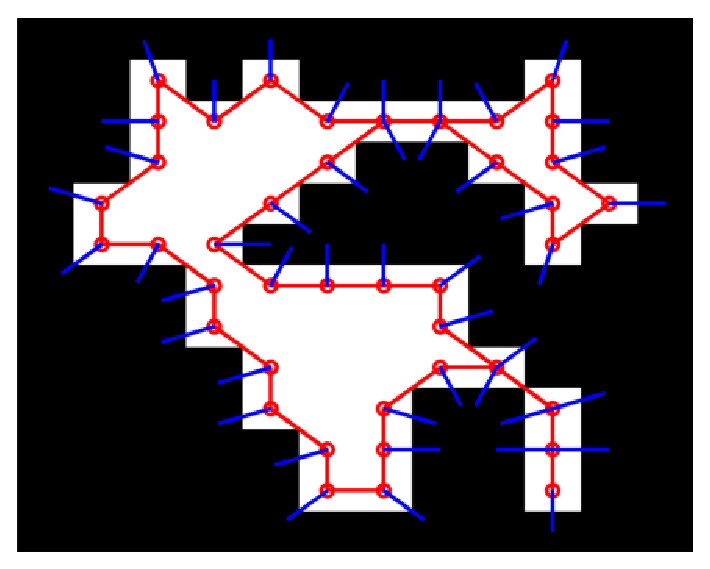
\includegraphics[width=7cm]{./pics/moore.eps}
\caption{Detection du voisinage externe d'une {\it figure}}
\label{fig:moore}
\end{figure}

Les contours d'une {\it figure} sont examinés dans le sens horaire en
utilisant l'algorithme du voisinage de Moore \cite{url-moore}. Cette
approche permet d'obtenir une liste triée des contours de chaque {\it
figure}.


\subsection{Conversion au format SVG}
Le format SVG permet de representer le contenu d'une image par le
comme étant plusieurs entités géométriques, par le biais de simples tags
{\it xml} \cite{url-svg}. Le type de figure le plus générique est
caractérisé par l'élément {\it path}. Un {\it path} est un "chemin"
permettant  de représenter n'importe quel type de figure comme étant
une suite de segments ou de courbes.

La traduction au format SVG n'est rien d'autre que la conversion en
{\it paths} des contours de chaque {\it figure}. L'unique inconvénient
de cette étape est la possibilité d'avoir des {\it
figures} superposés.  Pour éviter qu'une {\it figure} puisse cacher
une autre il est indispensable de trier les {\it figures} selon leur
taille et contenu. Les {\it figures} sont triées selon leur distance 
depuis les bords de l'image en utilisent le principe que, si une
{\it figure } est plus proche d'un bord de l'image qu'une autre,
alors la dernière ne pourra jamais couvrir la première.


\section{Valeurs optimales}
Tout au long du développement nous avons pu tester les algorithmes à
plusieurs reprises et surtout avec des valeurs d'option différentes,
influençant directement le qualité de l'image filtrer.
Fort des tests que nous avons réalisés, nous vous mettons à disposition
les valeurs des options qui présentent des résultats intéressant.

\begin{itemize}
\item Sobel: black thresh = 20 , white thresh = 150
\item Prewitt: black thresh = 20 , white thresh = 150
\item Kirsch: black thresh = 25 , white tresh = 155
\item Roberts: black thresh = 20 , white tresh = 220
\item Gauss: sigma = 1.2 , radius = 2
\item Canny: thresh min = 60 , thresh max = 220 , double thresh min = 60 , double thresh max = 220
\item Segmentation: nombre de couleur = 3
\item Cluster-edges: nombre de couleur = 3
\end


\newpage
\addcontentsline{toc}{section}{Références}
\bibliographystyle{plain}
\bibliography{rapport}

\end{document}
